%!TEX root = ../report.tex

\section{Kraft}

\begin{wrapfigure}{r}{0.5\textwidth}
    \begin{center}
        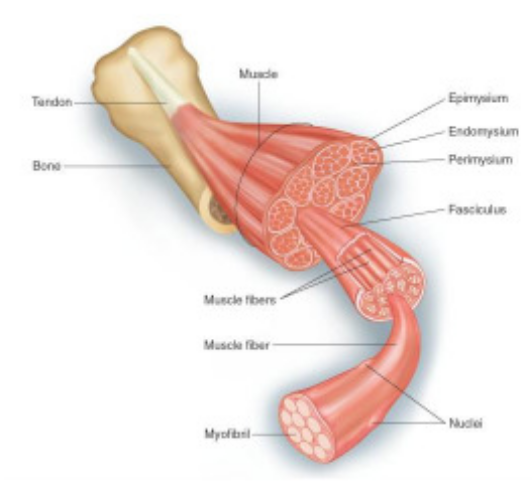
\includegraphics[width=0.48\textwidth]{pictures/muskeln}
    \end{center}
\end{wrapfigure}

Beispiele:
\begin{itemize}
    \item einmalig maximale Kraft (Gewichtheben)
    \item schnell und viel Kraft (Ringen, Hochsprung)
    \item Kraft aufrecht erhalten (Brücke)
\end{itemize}

Anatomische Grundlagen:
\begin{itemize}
    \item grundsätzlich drei Komponenten: Muskel, Sehne, Knochen
    \item Muskel bestehen aus:
    \begin{itemize}
        \item Muskelfaserbündel
        \item Muskelfaser
        \item Myofibrille
        \item Sarkomer
        \item Aktin-Myosin
    \end{itemize}
\end{itemize}

\begin{figure}[h]
\centering
\begin{tabular}{|c|c|c|c|}
 \hline
Kontraktionsform & Arbeitsweise & Ansatz / Ursprung & Beispiel Liegestütze \\ \hline \hline
konzentrisch & überwindend & Wird kleiner & Von Boden in Stütz \\ \hline
exzentrisch & nachgebend & Wird größer & Von Stütz auf Boden \\ \hline
isometrisch & haltend & Bleibt gleich & Halten des Stützes \\ \hline
\end{tabular}
\caption{Aktionsformen der Muskeln}
\end{figure}

\subsection{Struktur der Kraft}

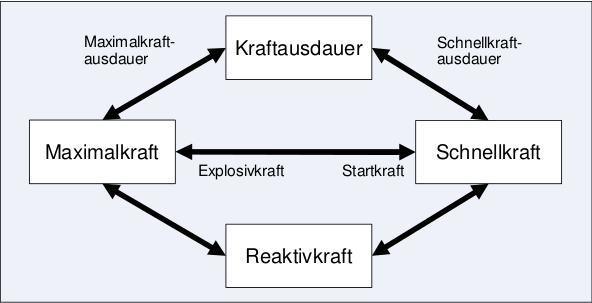
\includegraphics[width=\textwidth]{pictures/kraftstruktur}

\subsection{Determinanten der Kraft}
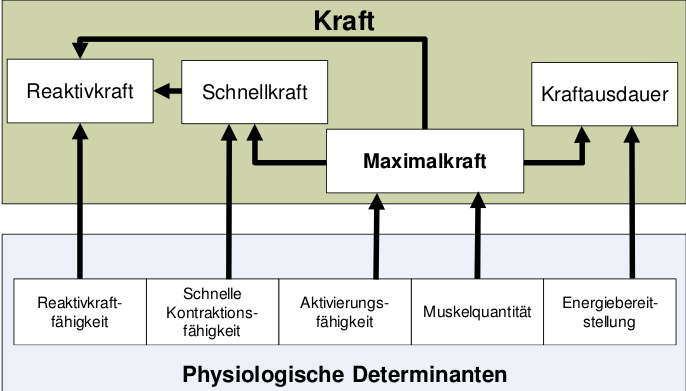
\includegraphics[width=\textwidth]{pictures/kraft_determinanten}

\subsection{Maximalkraft}

\begin{minipage}{0.5\textwidth}
\begin{itemize}
    \item Definition: Maximalkraft ist die höchstmögliche Kraft, die vom Nerv-Muskel-System willentlich gegen einen Widerstand erzeugt werden kann
    \item 1er-Maximum (1RM = 1 Repetition Maximum) = konzentrische Maximalkraft über volle Bewegungsamplitude
    \item Relativkraft = 1RM / Körpergewicht
    \item bestehend aus:
    \begin{itemize}
        \item Muskelquerschnitt \& Faserzusammensetzung
        \item Willkürliche Aktivierungsfähigkeit
    \end{itemize}
\end{itemize}
\end{minipage}
\begin{minipage}{0.5\textwidth}
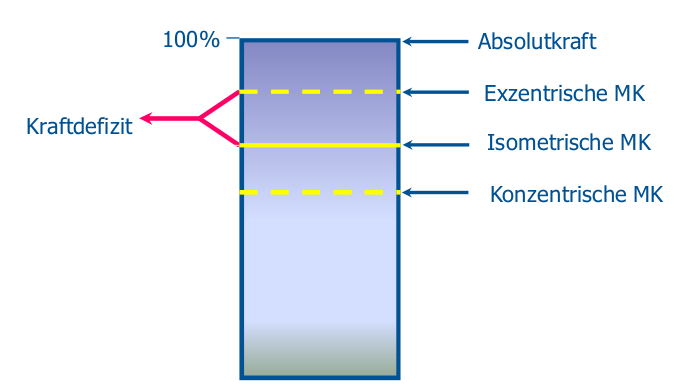
\includegraphics[width=1.1\textwidth]{pictures/maximalkraftvarianten}
\end{minipage}

\begin{itemize}
    \item Absolutkraft: Nur durch maximale elektrische Stimulation erreichbare Kraft. Willentlich nicht abrufbar.
    \item Kraftdefizit: $\frac{\text{Exzentrische MK} - \text{Isometrische MK}}{\text{Exzentrische MK}} \cdot 100 \%$
    \item in Praxis: Differenz zwischen isometrischer und exzentrischer MK
    \item Training:
    \begin{itemize}
        \item großes Kraftdefizit: willkürliche Aktivierungsfähigkeit verbessern
        \item kleines Kraftdefizit: Muskelquantität
    \end{itemize}
\end{itemize}

\subsection{Schnellkraft}

\begin{minipage}{0.5\textwidth}
\begin{itemize}
    \item Definition: Schnellkraft ist die Fähigkeit, einen möglichst großen Kraftstoß innerhalb einer zur Verfügung stehenden (kurzen) Zeit zu realisieren
    \item Teilaspekte:
    \begin{itemize}
        \item Startkraft (Fähigkeit sehr schnell Kraft zu entfalten, bsp: Boxen?)
        \item Explosivkraft (Fähigkeit großen/schnellen Kraftanstieg zu realisieren, bsp: Würfe, Stöße, Schüsse?)
        \item Dynamisches Kraftmaximum (Fähigkeit MK schnell zu realisieren, bsp: Ringen?)
    \end{itemize}
\end{itemize}
\end{minipage}
\begin{minipage}{0.5\textwidth}
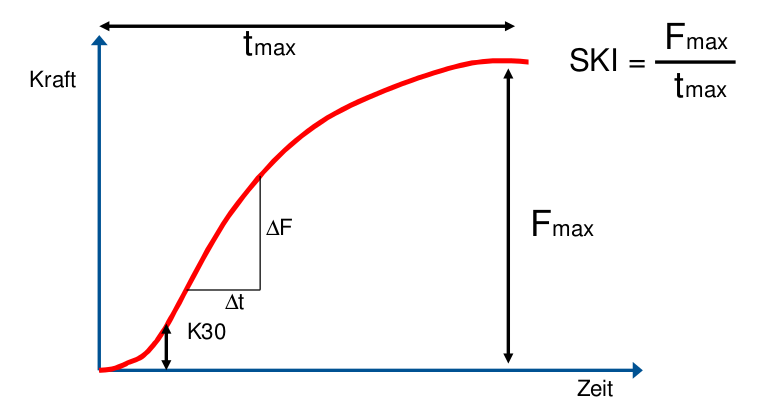
\includegraphics[width=\textwidth]{pictures/kraftanstiegskurve}
\end{minipage}
\begin{itemize}
    \item Struktur der Schnellkraft: Maximalkraft + Schnelle Kontraktionsfähigkeit
    \item Schnelle Kontraktionsfähigkeit hängt ab von Muskelfaserzusammensetzung, Intermuskulärer und Intramuskulärer Koordination
\end{itemize}

\paragraph{Muskelfaserzusammensetzung}
\begin{itemize}
    \item Zusammensetzung genetisch determiniert
    \item Umwandlung praktisch nur Fast Twitch to Slow Twitch durch Ausdauertraining und Querschnittstraining
\end{itemize}
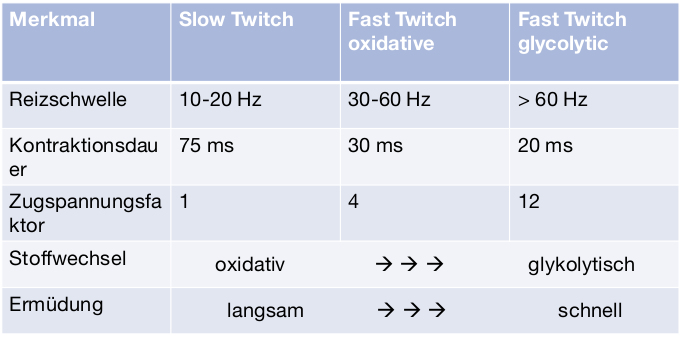
\includegraphics[width=\textwidth]{pictures/muskelfaserzusammensetzung}

\paragraph{Intermuskuläre Koordination}
\begin{itemize}
    \item Zusammenspiel mehrerer Muskeln (Muskelabschnitte)
    \item fertigkeitsspezifisch
    \item kann als Synonym für ``Gute Technik'' betrachtet werden
    \item Grund warum Krafttraining nicht nur auf Stärkung der einzelnen Muskeln ausgelegt sein darf
    \item Beispiele: Fuß-, Knie- und Hüftstrecker bei Strecksprung
\end{itemize}

\subsubsection*{Intramuskuläre Koordination}

\begin{minipage}{0.6\textwidth}
\begin{enumerate}
    \item Sequenzierung: Optimale Reihenfolge der Innervation der Muskelfasern
    \item Frequenzierung: Fähigkeit, den Muskel hochfrequent und nachhaltig zu innervieren
    \begin{itemize}
        \item Je nach Stärke der Erregung über die spinalen Synapsen, feuert ein Motoneuron mit unterschiedlicher Frequenz
        \item  Ab 55 Hz wird Maximale Kraftabgabe möglich
        \item  Bis zu 155 Hz sind möglich und erlauben schnellen Kraftanstieg
    \end{itemize}
    \item Rekrutierung: Fähigkeit, möglichst viele motorische Einheiten zur Kontraktion heranziehen zu können
    \begin{itemize}
        \item bei Kontraktion sind nie alle anatomisch vorhandenen Muskelfasern beteiligt
        \item Bei niedrigen Belastungen werden schwache, langsame, aber ausdauernde Einheiten angeschaltet
        \item Bei höheren dann auch die Starken und Schnellen!
    \end{itemize}
\end{enumerate}
\end{minipage}
\begin{minipage}{0.4\textwidth}
    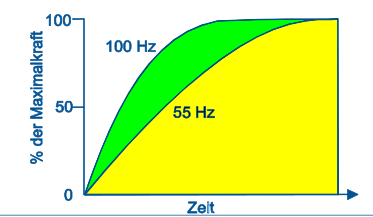
\includegraphics[width=\textwidth]{pictures/frequenzierung}
    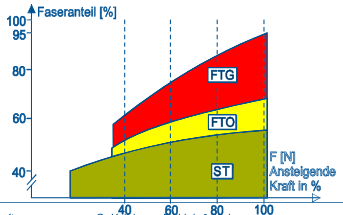
\includegraphics[width=\textwidth]{pictures/rekrutierung}
\end{minipage}

\subsection{Kraftausdauer}

\begin{itemize}
    \item geteilt in statisch und dynamische Kraftausdauer
    \item \textbf{Definition}: Kraftausdauer ist die Fähigkeit des neuromuskulären Systems, eine möglichst hohe Kraftstoßsumme in einer gegebenen Zeit zu produzieren
    \item Abgrenzung zur Ausdauer: Bewegungsintensität >50\% der Maximalkraft und Ausdauer ist führende Komponente (trotz Hypertrophieschwelle bei ca. 30 \%)
    \item \textbf{Definition ``Statische KA''}: ... ist die Fähigkeit, den Spannungsverlust (eines/ meherer Muskels/-n) über eine gegebene Zeit möglichst gering zu halten
    \item \textbf{Definition ``„Dynamische KA''}: ...ist die Fähigkeit, bei wiederholten Kraftstößen über einen gegebene Zeit die Verringerung dieser Kraftstöße möglichst gering zu halten
\end{itemize}

 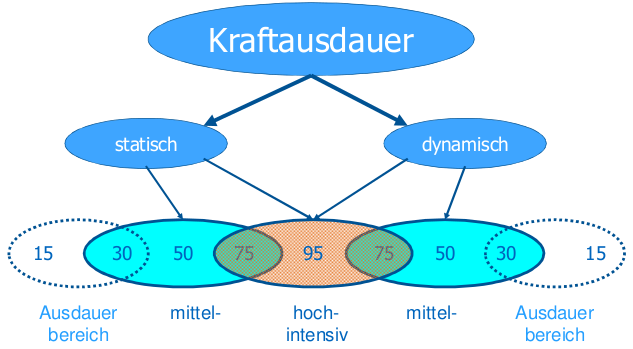
\includegraphics[width=\textwidth]{pictures/kraftausdauer}

 \subsection{Reaktivkraft}

 \begin{itemize}
    \item Definition: Reaktivkraft ist die Fähigkeit, in einem Dehnungs-Verkürzungs-Zyklus (DVZ) einen möglichst hohen Kraftstoß zu realisieren
    \item Definition DVZ: Schneller Wechsel (kleiner 170ms) von exzentrischer und konzentrischer Arbeitsweise
    \item Beispiele: Springen, Sprinten, „Peitschbewegung“
    \item Sportler mit hoher Reaktivkraft weisen ein spezielles Innervationsmuster auf und verfügen über die Fähigkeit, mechanische Energie im Gewebe elastisch zwischen zu speichernbei Schlägen und Würfen
    \item geteilt in Maximalkraft, Reaktive Spannungsfähigkeit und schnelle Kontraktionsfähigkeit
    \item Reaktive Spannungsfähigkeit:
    \begin{itemize}
        \item Passive Elastizitätskräfte Muskeln und Sehnen
        \item Zusätzliche neuronale Aktivierung
        \item DVZ: Kurze (< 170 ms) und lange (> 170 ms) DVZ und entsprechend Akzente in der Determination
    \end{itemize}
\end{itemize}

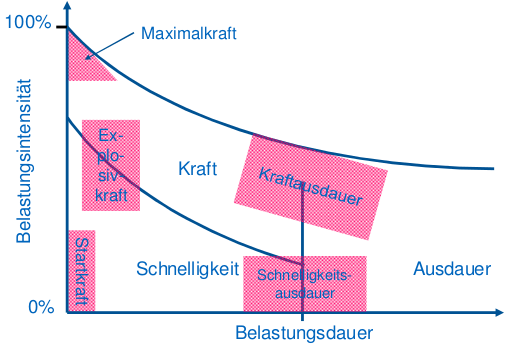
\includegraphics[width=0.90\textwidth]{pictures/landkarte}

\subsection{Krafttraining}

\begin{itemize}
    \item Definition: Verwendung von freien Hanteln, Maschinen, des eigenen Körpergewichts oder von Gummibändern zur Erzeugung eines zu überwindenden Gegenstandes
    \item Ziel: Ansteuerung des Leistungspotential
    \item Belastungsnormatives Krafttraining:
    \begin{itemize}
        \item Intensität (=Last): Abstufung nach \% des 1 RM: maximal (100), submaximal (99-80), mittel (80-65), leicht (65-50), gering (50-30)
        \item Dauer (=Wiederholungen): unmittelbar hintereinander ausgeführte Kontraktionen
        \item Umfang (=Serien=Sätze): z.B. 3 Sätze á 10 Wiederholungen.
        \item Dichte (=Pausen): Pause zwischen Wiederholungen bzw. Sätzen
        \item Arbeitsweise: Kontraktionsform: konzentrisch, exzentrisch, isometrisch Bewegungsgeschwindigkeit: explosiv, zügig, mittel, langsam
        \item Organisationsform: Satztraining, Zirkeltraining
    \end{itemize}
\end{itemize}

\subsection{Trainingsmethoden}

\subsubsection*{Determinanten Quantität}

\begin{minipage}{0.3\textwidth}
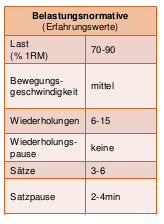
\includegraphics[width=0.9\textwidth]{pictures/hypertrophiemethode}
\end{minipage}
\begin{minipage}{0.7\textwidth}
\begin{itemize}
    \item 1 cm 2 Muskelquerschnitt liefert ca. 65 Newton
    \item Hypertrophie (lat. „Überernährung“) meint Dickenwachstum der Muskelfasern durch erhöhte Proteinsynthese
    \item Ursache 1: Mechanischer Stress (Verletzung der Muskelfaser durch mechanische Überbelastung) $\rightarrow$ Hohe Lasten (Muskelspannungen) zum Hervorrufen von Mikrotraumata erforderlich
    \item Ursache 2: Metabolischer Stress (Hypoxische Nebenprodukte infolge energetischer Verausgabung) $\rightarrow$ Hohe Leistungsabgabe zum Ausschöpfung der Phosphatspeicher erforderlich
    \item Hypertrophiemethode:
    \begin{itemize}
        \item „Methode der erschöpfenden submaximalen Krafteinsätze“
        \item submaximal
        \item bei zu hoher Last keine metabolische Ausbelastung
        \item bei zu geringer Last keine Mikrotraumata
        \item Wiederholungen bis zum lokalen Muskelversagen
        \item keine Pause zwischen Wiederholungen
    \end{itemize}
\end{itemize}
\end{minipage}

\subsubsection*{Determinanten Aktivierungsfähigkeit}

\begin{itemize}
    \item Qualität der Intramuskulären Koordination (IK)
    \item Rekrutierungsmuster (langsame Kraftentwicklung)
    \begin{enumerate}
        \item Rekrutierung: Beteiligung einer zunehmenden Anzahl motorischer Einheiten, Vollständige Rekrutierung bei ca 90\% der MK
        \item Frequenzierung: Steigerung der Entladungsfrequenz der Motorneurone, Maximale Frequenzierung bei ca. 98\% MK
        \item Synchronisation: Gleichzeige elektrische Entladung der Motorneurone $\rightarrow$ sehr hohe Lasten ($\ge 90 \%$ erforderlich)
    \end{enumerate}
\end{itemize}

\begin{minipage}{0.3\textwidth}
    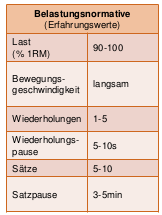
\includegraphics[width=0.9\textwidth]{pictures/ik-methode}
\end{minipage}
\begin{minipage}{0.7\textwidth}
    IK-Methode:
    \begin{itemize}
        \item „Methode der explosiven maximalen Krafteinsätze“
        \item (fast) maximal
        \item folglich sehr wenige Wiederholungen
        \item Wiederholungspause bis zur Regeneration der Phosphatspeicher, sonst Übersäuerung
        \item Krafteinsatz erfolgt explosiv Bewegungsgeschwindigkeit ist, de facto langsam
        \item Satzpause bis Wiederherstellung der (fast) vollen Funktionsfähigkeit
    \end{itemize}
\end{minipage}

\subsubsection*{Determinanten schnelle Kontraktionsfähigkeit}

\begin{minipage}{0.3\textwidth}
    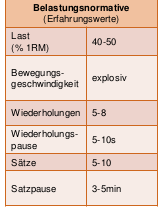
\includegraphics[width=0.9\textwidth]{pictures/schnellkraftmethode}
    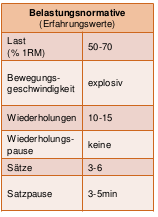
\includegraphics[width=0.9\textwidth]{pictures/schnellkraftorientierte_hypertrophiemethode}
\end{minipage}
\begin{minipage}{0.7\textwidth}
    \begin{itemize}
        \item Muskelfasertypen: Slow-Twitch (ST), Fast-Twitch oxidative (FTO), Fast-Twitch glycolytic (FTG)
        \item Rekrutierungsmuster (explosiver Krafteinsatz): nahezu gleichzeitige Rekrutierung aller Fasertypen, aber der Hauptbeitrag wird wegen ihrer geringerem Verkürzungsgeschwindigkeit von den FT-Fasern geleistet $\rightarrow$ Schnelle Kontraktionsfähigkeit ist von Quantität \& Intramuskulären Koordinaten der FT-Fasern abhängig
        \item Schnellkraftmethode
        \begin{itemize}
            \item „Methode der explosiv-ballistischen Krafteinsätze“
            \item Bewegungsgeschwindigkeit (fast) maximal bei explosivem Krafteinsatz
            \item ballistisch = Bewegung endet mit Kontraktion ohne Wiederstand
            \item Last so das fast max. Geschwindigkeit möglich ist
            \item Wiederholungspause bis zum Auffüllen der ATP-Speicher
            \item Abbruch eines Satzes bei deutlichem Geschwindigkeitsverlust
        \end{itemize}
        \item schnellkraftorientierte Hypertrophiemethode:
        \begin{itemize}
            \item „Methode der erschöpfenden kontinuierlich-schnellen Krafteinsätze"
            \item Bewegungsgeschwindigkeit: so schnell wie möglich bei explosiver Krafteinsatz, de facto: nicht maximal
            \item Last angepasst, höher als bei Schnellkraftmethode
            \item Abbruch eines Satzes bei deutlichem Geschwindigkeitsverlust
        \end{itemize}
    \end{itemize}
\end{minipage}

\subsubsection*{Physiologische Grundlagen Reaktivkraft}

\begin{minipage}{0.3\textwidth}
    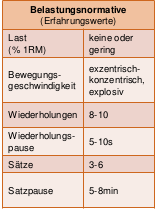
\includegraphics[width=0.9\textwidth]{pictures/reaktive_methode}
\end{minipage}
\begin{minipage}{0.7\textwidth}
    \begin{itemize}
        \item Reaktivkraft ist abhängig von der Fähigkeit des Gewebes mechanische Energie zu speichern (stiffness, reaktive Spannungsfähigkeit), Maximalkraft und Schnellkraft
        \item Reaktive Methode:
        \begin{itemize}
            \item „Methode der reaktiven Krafteinsätze"
            \item kurzer Bremsweg und schnelle Umkehrphase (Ziel <200ms)
            \item exzentrische Kraftwirkung muss von Muskulatur, nicht vom passiven Bewegungsapparat aufgenommen werden
            \item Bewegungsgeschwindigkeit in konzentrischer Phase explosiv
            \item DVZ insgesamt so kurz wie möglich gestalten
            \item keine oder geringe Last
            \item Abbruch, wenn keine reaktive Arbeitsweise mehr möglich ist
        \end{itemize}
    \end{itemize}
\end{minipage}

\subsubsection*{Energiebereitstellung / Physiologische Grundlagen Kraftausdauer}

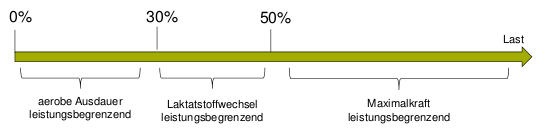
\includegraphics[width=0.9\textwidth]{pictures/kraftausdauer_bar}

Kraftausdauer = zwischen 30\% und 60\% der MK $\rightarrow$ Training in einem Intensitätsbereich an dem Laktatstoffwechsel die Leistung begrenzt

\begin{minipage}{0.3\textwidth}
    \begin{itemize}
        \item Muskelleistungsschwelle: Bereich, in dem der Muskel die größte Leistung abgibt (Kraft * Geschwindigkeit)
        \item Fähigkeit zur Aufrechthaltung einer hohen Muskelleistung in vielen Sportarten leistungsbegrenzend
    \end{itemize}
\end{minipage}
\begin{minipage}{0.7\textwidth}
    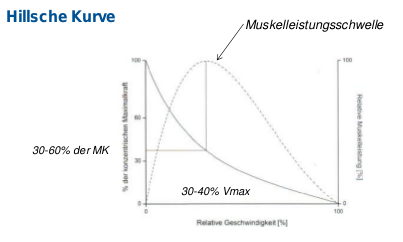
\includegraphics[width=0.9\textwidth]{pictures/hillsche_kurve}
\end{minipage}

\begin{minipage}{0.3\textwidth}
    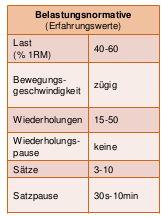
\includegraphics[width=0.9\textwidth]{pictures/kraftausdauermethode}
\end{minipage}
\begin{minipage}{0.7\textwidth}
Kraftausdauermethode:
\begin{itemize}
    \item „Methode der erschöpfenden maximalen Muskelleistung"
    \item Last an Muskelleistungsschwelle
    \item Bewegungsgeschwindigkeit zu beginn so hoch wie an Muskelleistungsschwelle möglich (alternative statisch)
    \item Wiederholungen bis zur lokalen Muskelerschöpfung, mehr als bei Hypertrophiemethode
\end{itemize}
\end{minipage}

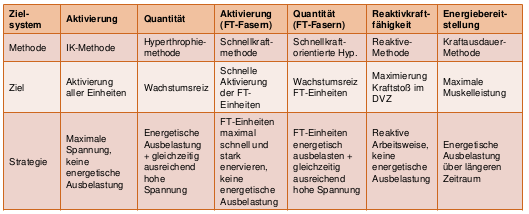
\includegraphics[width=0.9\textwidth]{pictures/zusammenfassung_kraft_methoden}

\subsubsection*{Periodisierung}

\begin{minipage}{0.7\textwidth}
    Aufbauzyklus:
    \begin{itemize}
        \item zunächst Maximalkraft
        \item bei hohem Kraftdefizit (ca. 35\%) Aktivierung
        \item bei geringem Kraftdefizit (ca. 10\%)Quantität
        \item danach führenden Kraftkomponente je nach je Sportart (Kraftausdauer, Schnellkraft, Reaktivkraft
    \end{itemize}

    Wettkampfzyklus:
    \begin{itemize}
        \item moderates Training der führenden Kraftkomponente
        \item  Achtung: Intensives Hypertrophietraining kann sich negativ auf Schnellkraft auswirken
    \end{itemize}
\end{minipage}
\begin{minipage}{0.3\textwidth}
    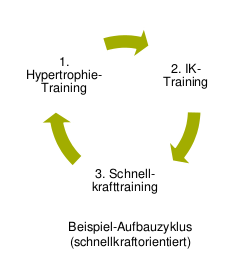
\includegraphics[width=0.9\textwidth]{pictures/bsp_aufbauzyklus}
\end{minipage}

\subsection{Trainingsinhalte}

Allgemeines Krafttraining:
\begin{itemize}
    \item Training (global) der bewegenden Muskeln
    \item Aufbau von Kraftfähigkeiten (zumeist der Hauptmuskelgruppen)
    \item sportartunabhängige Übungen
    \item Beispiele: Arnold Press, Latzug, Langhantelrudern, Kniebeuge, Bankdrücken, Beincurls, ...
\end{itemize}

Spezifisches Krafttraining:
\begin{itemize}
    \item Training mit Nähe zur Zielbewegung
    \item Problem: Übung führt primär zu Leistungssteigerungen bei der Übung
    \item Kraftfähigkeiten sind sportartspezifisch!
    \item Krafttraining darf nicht nur auf Stärkung der einzelnen Muskeln ausgerichtet sein, sondern auch auf eine Verbesserung der intermuskulären Koordinaten ("gute Technik").
    \item Ansatz 1:
    \begin{itemize}
        \item Grundübungen mit gleichem Gelenkwinkel und gleicher Kontraktionsform wie in Zielbewegung
        \item Kritik: teilweise experimentell widerlegt und Ausbelastung führt zu großer mechanischer Belastung
    \end{itemize}
    \item Ansatz 2:
    \begin{itemize}
        \item keine Grundübung sondern Zielbewegung mit Zusatzlast
        \item Kritik: Evtl. Veränderung der Bewegung bei zur großem Gewicht und bei ausreichend hohem Widerstand u.U. gefährlich!!
    \end{itemize}
    \item Ansatz 3:
    \begin{itemize}
        \item Kraft mit Grundübung aufbauen und Transfer getrennt trainieren
        \item Hauptargument: Effektivität des Kraftreizes ist wichtiger als Nähe zur Bewegung
    \end{itemize}
\end{itemize}

Stabilitätstraining:
\begin{itemize}
    \item Training (lokal) stabilisierender Muskeln
    \item SPÄTER!
\end{itemize}

\subsection{Anwendung}
Ziele nach Anwendungsfeld: \\

\begin{tabular}{m{0.4\textwidth} | m{0.18\textwidth} |  m{0.4\textwidth}}
    Leistungssport mit Kraft als wichtige Teilfähigkeit & maximierend / \newline optimierend & alle für die Fähigkeit relevanten Methoden und Inhalte \\
    Sonstiger Leistungssport & unterstüzend & Allgemeines Krafttraining, Stabilisierung \& Hypertrophie \\
    Gesundheitssport, Kinder- und Jugendkrafttraining & gesundheitsfördernd & ``Sanftes Krafttraining'', Stabilisierung \\
\end{tabular}
\\

``Sanftes'' Krafttraining:
\begin{itemize}
    \item 10-15 (max. 6-25) Wiederholungen
    \item keine Ausbelastung, langsame Ausführung
    \item zunächst nur einen Satz, später bis zu 3
    \item 6-8 Übungen
    \item Bauch \& Rücken zuerst
    \item 2 mal pro Woche, 6-8 Wochen, 2 Zyklen pro Jahr
    \item Im Kindersport lange kritisch gesehen, heute wird altersangepasstes Krafttraining ab ca. 7 Jahren empfohlen
\end{itemize}

\subsection{Diagnostik}
Allgemeine Kraftdiagnostik:
\begin{itemize}
    \item Sportmotorische Tests, z.b. Liegestütz, Klimmzüge, Situps haben häufig Messprobleme
    \item Exaktere Bestimmung über Kraftmaschinen
    \begin{itemize}
        \item 1 RM (im Freizeitbereich kritisch)
        \item 5 RM (hochrechnen auf 1 RM, ca. 80\%)
        \item Spezielle Maschinen (z.B. Fa. Cybex) registrieren Kraft, die man bei einer konstanten Winkelgeschwindigkeit aufbringen kann
    \end{itemize}
    \item Diagnostische Aussagen: Maximalwerte, Verläufe über Winkelbereich, Symmetrien
\end{itemize}
Sportartspezifische Krafttests:
\begin{itemize}
    \item Beispielbatterie Sprungkraft für Volleyball: Squat Jump, Counter Movement Jump, Counter, Covement mit Armen, Blocksprung, Angriffsschlag, 10 Angriffsschläge in Folge
    \item Diagnostische Aussagen: Absolutes Niveau pro Test (Relativ zur Mannschaft / Normen oder Relativ zu früheren Testzeitpunkten (Trainingsauswertung)), Relation der Tests untereinander (Lokalisation von Stärken/Schwächen)
\end{itemize}

\subsection{Zusammenfassung}
\begin{itemize}
    \item Physiologische Grundmechanismen determinieren Methodik
    \item Sehr gut ansteuerbar in jedem Lebensalter
    \item Schwierigkeit ist der Transfer in die Zielbewegung $\rightarrow$ Kombination verschiedener Strategien
    \item Positive gesundheitliche, ästhetische, psychische Wirkungen bei richtiger Dosierung
\end{itemize}
